\section{Crowd Conditions}\label{sec:related_work}

When people gather in crowds, conditions develop that are beyond the deliberate actions of the individuals. These conditions are referred to as crowd conditions. At large events and gatherings the personnel should be aware of the crowd conditions, as they must be able to decide when, where, and how they need to intervene in order to ensure the safety and comfort of the crowd.

This section will first outline some conditions that are hazardous or have potential to evolve into such. Afterwards it will cover crowd characteristics, that when observed can supply the personnel with information which will help them predict, prevent and dissolve hazardous crowd conditions.

\subsection{Hazardous Crowd Conditions}
Large crowds are intrinsically dangerous, as the effects of individual people's actions combine into great forces, which the individuals are not aware of~\cite{website:Wikipedia-Hajj}. Some of these conditions are:

\begin{enumerate}
    \item Stampedes - Which in this report refers to \enquote{a collective movement towards or away from a place caused by a common reaction to said place}. Examples of this could be the evacuation of a building on fire~ \cite{website:Wikipedia-stationclubfire}, or pilgrims trying to reach their destination ~\cite{website:Wikipedia-minastampede}. Although stampedes can be violent, fast moving and cause death by trampling, the main cause of death is compressive asphyxia\footnote{Oxygen starvation caused by compression of the torso inhibiting breathing} typically caused by an immense pressure~\cite{fruincauses}.
    
    \item Congestion - This is an involuntary reduction in the flow of a crowd, which is the rate of people passing through an area. This reduction can be caused by opposing movements in the crowd, or a buildup of impassable objects such as bodies~\cite{ website:Wikipedia-stationclubfire,website:Wikipedia-meccatunnel}. A complete congestion in this report will refer to a condition in the crowd where the only movement is involuntary. The alternative is where the crowd can still move voluntarily but with involuntary slowdown.
    
    %\item Crowd psychology - physical crowds vs. psychological crowd. undlader at nævne crowd psychology her, da vi ikke kommer ind på det efterfølgende.
    
    \item Stop and go waves - Which is a form of irregular movement in the crowd. It is caused by a drop in the flow of the crowd. If the drop in the flow is significant, temporary congestion can occur which forces people to stop their movement completely, causing a rippling effect which propagates backwards through the crowd, which in turn causes pressure to build, as people stop their movement against the crowd. This kind of movement can cause people to fall over, as they are pushed around, or cause compression of the crowd~\cite{empircalstudy,videoanalysis}.
    
    \item Crowd Panic - Is a state in which the crowd experiences discomfort to such a level that they will disregard normal social behaviour in order to relieve their discomfort. Examples would be attempts to push other people away in order to gain breathing space or violently trying to pass through the masses in an attempt to vacate the area~\cite{empircalstudy}. An example of this would be the LoveParade incident of 2010~\cite{loveParadeDisaster}.
\end{enumerate}

%%%%%%%%%%%%%%%%%%%%%%%%%%%%%%%%%%%%%

%\cite{wirz2012inferring}
%\enquote{In the case of an actual crowd control situation or emergency, information about jammed exits or passageways is critical to the deployment of appropriate countermeasures.}

%\enquote{As stated by the interviewees, the ability to identify potential crowd management issues from CCTV footage requires that the CCTV operator is able to recognise the possible indicators of these issues and has a high level of concentration during the event.}

%\enquote{In a preceding study, we have verified that people are willing to share privacy-sensitive location information if they receive some benefits or if they realise that sharing such information is for their own good and safety [12]}

%\enquote{To collect location information of festival attendees, we developed a generic festival app for mobile devices which can be tailored to a specific event and provides the users with relevant, event-related information such as the festival program, a map indicating points of interest and background information. These features are designed to be attractive and useful during the event to reach a large user base. While a user is running the app, GPS location is regularly sampled with a frequency of 1Hz on the device and periodically sent to our servers running the CoenoSense}

%\enquote{Having an estimated number of the actual crowd density, would be preferred}
\subsection{Crowd Condition Characteristics}

The condition of a crowd and its effect on safety and comfort can be difficult to deduce, even if event organisers and their safety staff are well educated~\cite{franke2015smart}. Even if a hazard is discovered it may be too late to prevent an oncoming accident. Because of this, it is important to be aware of preconditions of a developing hazard as early as possible, so that appropriate action can be taken.

In \citet{wirz2012inferring}, four distinct characteristics were found that can be used to infer crowd conditions; density, velocity, turbulence and pressure.

\subsection{Density}
Density is the amount of people relative to available space. In this project we will look at $\text{people} / m^2$, but it is important to keep in mind that it is possible to expand to other measures of available space.

Density can be a good indicator for inferring hazardous situations. For instance most stampedes occur in high-density crowds~\cite{wirz2012inferring}. Research has determined  certain density limits for still-standing crowds, where it becomes highly uncomfortable to be in. 
Density can however also be misleading with regards to safety and comfort. For instance people standing tightly packed inside a metro train can often tolerate standing a lot closer, than when moving down the subway stairs during rush hour. When illustrating density with the purpose of observing the safety and comfort in the crowd, it is important that this is not the only information available.

If a hazardous situation has been predicted or observed, density can be an important factor to observe. Density can have an impact on the accessibility of an area. In \citet{wirz2013probing} it was found that the density of the people in an area has a direct effect on how fast people can comfortably move within it. They use it to predict the density of the crowd from an observed local crowd velocity. This could therefore also be used to predict how fast a person generally moves through a crowd using observed densities. Because of this, density can help the personnel to better plan how to access a potentially hazardous area.

The specific pros and cons of density as a crowd condition is summarised in \cref{sec:crowd_conditions_summary}.

\subsection{Movement Velocity and Heading Direction}
The safety and comfort of a crowd does not only depend on density, but also on the movement in a crowd. Movement in a crowd can be split up into two categories, where people are heading, and what their velocity is.

\subsubsection{Crowd Velocity}
We use the standard concept of velocity, i.e. the direction people are moving and the magnitude of that movement. Specifically we use the SI unit of a vector in meters per second to depict the movement of individual people. The velocity of an individual at time $t$ is the vector given by the last two observations, $t$ and $t-1$, projected onto time $t$. We can use the velocity of individual people in an area to find the local crowd velocity. The local crowd velocity is the estimated velocity of a crowd at a specific point, and can be seen illustrated in \cref{fig:localCrowdVelocity}.

\begin{figure}[htbp]
\centering
\begin{subfigure}[t]{0.48\linewidth}
\centering
\begin{tikzpicture}[framed]
\coordinate(P) at (0,0);
\coordinate(P') at (1,0);
\coordinate(A) at (0.25,1);
\coordinate(A') at (1.25,1);
\coordinate(B) at (-0.3,-1);
\coordinate(B') at (0.7,-1);
\coordinate(C) at (-1.5,0.5);
\coordinate(C') at (-0.5,0.5);

\draw[->, thick] (A) -- (A');
\draw[->, thick] (B) -- (B');
\draw[->, thick] (C) -- (C');
\draw[->, thick] (P) -- (P');

\filldraw[color = red]
(A) circle (2pt)
(B) circle (2pt)
(C) circle (2pt);

\filldraw[color = blue]
(P) circle (3pt);
\draw (P) node[anchor=south west] {Local Crowd Velocity};

\end{tikzpicture}
\caption{Uniform velocity - Everyone is moving in the same direction with the same speed, so the local crowd velocity matches this velocity.}
\end{subfigure}
\quad
\begin{subfigure}[t]{0.48\linewidth}
\centering
\begin{tikzpicture}[framed]
\coordinate(P) at (0,0);
\coordinate(P') at (0.66,0);
\coordinate(A) at (0.25,1);
\coordinate(A') at (1.25,1);
\coordinate(B) at (-0.3,-1);
\coordinate(B') at (-1.3,-1);
\coordinate(C) at (-1.5,0.5);
\coordinate(C') at (-0.5,0.5);

\draw[->, thick] (A) -- (A');
\draw[->, thick] (B) -- (B');
\draw[->, thick] (C) -- (C');
\draw[->, thick] (P) -- (P');

\filldraw[color = red]
(A) circle (2pt)
(B) circle (2pt)
(C) circle (2pt);
\filldraw[color = blue]
(P) circle (3pt);
\draw node[anchor=south west] {Local Crowd Velocity};

\end{tikzpicture}
\caption{Nonuniform velocity - The majority of the people move in the same direction with same speed. The rest of the crowd moves in the opposite direction with the same speed as the majority of the crowd. The local crowd velocity is the same direction as the majority, but with a lesser speed in that direction.}
\end{subfigure}
\caption[Local crowd velocity illustration]{An illustration of the local crowd velocity in different situations. Red points symbolises people with a direction and speed. The blue dots symbolises the local crowd velocity in the area.}
\label{fig:localCrowdVelocity}
\end{figure}

Local crowd velocity can be understood as the general velocity of the crowd in the point, and tries to capture how a person would feel the general velocity of the crowd being present in that point. It also tries to capture the most probable velocity the people in the crowd has, and therefore can be used to predict where people generally are moving.

Certain conditions of a crowd can have a direct effect on how fast people can pass through it. When navigating in such a crowd the shortest route to your destination may therefore not be the fastest.

The local crowd velocity can then be used to predict where the crowd, or specific parts of the crowd, is heading and to an extension how the crowd conditions will change. For example, if two crowds are moving towards each other and their combined density will exceed the capacity of their collision point, it is reasonable to expect congestion in that point, however there is no guarantee that people will not change direction. 

% Crowd’s movement velocity. The local crowd velocity can be seen as the weighted average velocity of each user at a given location by weighting the speed values of each user depending on the distance to that location with a Gaussian weighting scheme. <--- Useful sentence for later, BUT it has been copied, not written ourselves!

The specific pros and cons is summarised in \cref{sec:crowd_conditions_summary}.

\subsubsection{Heading Direction}\label{subsubsec:headingDirection}
People can change their velocity quickly and drastically. They often have a goal, and the best way to reach that goal is not necessary to set a heading straight for it, due to objects being in the way or other inconvenient obstacles. Because of this, \citet{wirz2012inferring} based on work of \citet{localTrendStatistics} introduced the concept of heading direction of individuals. Instead of expecting people to move according to their velocity we expect them to move according to how they have moved over the last couple of observations. In other words, we expect peoples direction of movement to be the average angle with which they have changed their direction of movement over previous observations. This is called heading direction and is illustrated in \cref{fig:headingvsvelocity}. The illustration shows the movement of a person, currently present in point t. $v$ is the velocity of the person over the last two observations, $t$ and $t-1$, and $h$ the heading direction of the person over all observations in the example, $t-4$ through $t$. In this example we can imagine that the person is moving around a obstacle to reach the other side. In order to reach tho other side of the obstacle the person will have to continue to move around the obstacle, i.e. continue according to their heading direction.

The heading direction is useful based on the assumption that the person is most likely to continue his or her movement at any given time. Note that the heading direction is not the same as averaging over all vectors in an observation, for example, averaging over all vectors in, $t-4$ through $t$, will only bring the resulting vector further from the heading direction.

\begin{figure}\centering
\begin{tikzpicture}
\circoord{0}{3}{3}{-90} {A};
\circoord{0}{3}{3}{-60} {B};
\circoord{0}{3}{3}{-30} {C};
\circoord{0}{3}{3}{0} {D};
\circoord{0}{3}{3}{30} {E};
\circoord{0}{3}{3}{60} {F};

\filldraw
(A) circle (2pt) node[above] {$t - 4$}
(B) circle (2pt) node[above] {$t - 3$}
(C) circle (2pt) node[right] {$t - 2$}
(D) circle (2pt) node[right] {$t - 1$}
(E) circle (2pt) node[right] {$t$};

\draw (A) arc (-90:30:3);
\draw[thick, ->] (E) arc (30:60:3) node[below] {$h$};

\draw[dashed] (D) -- (E);
\draw[thick, ->] (E) -- node[above right] {$v$} (2.196, 6);
\end{tikzpicture}
\caption{Example of difference between heading direction and velocity}
\label{fig:headingvsvelocity}
\end{figure}

\subsection{Turbulence}
\label{sub:crowdFactorTurbulence}
The concept of local crowd turbulence was first introduced by \citet{videoanalysis} and is the irregularity in the heading direction of the crowd. This means that a point in a crowd where people are moving in a lot of different directions will have a higher turbulence than one where people are more uniform in their movement. It is based on on the heading direction rather than the local crowd velocity, since heading direction is more precise in illustrating where individual people are heading towards. The more variance there is in heading directions of the people in the crowd the more unsettled people get, increasing the risk of people falling and crowd panic. This factor has been found to be good as an early indicator for hazardous situations in a crowd, especially in crowds with a low density\cite{wirz2012inferring}.

%Turbulence can be hard to infer from visual observations. The severity of the situation is also hard to observe without any form of calculations. Here a mobile based system with specific positions over time for the users, can do this a lot easier, since the velocity is easily observed here and calculations for turbulence can then be done before visualising it for the user.

\subsection{Pressure}
The pressure is the variance of the local crowd velocity times the local crowd density, and was suggested by \citeauthor{empircalstudy} \citeyearpar{empircalstudy} \cite{empircalstudy} and \citeauthor{videoanalysis} \citeyearpar{videoanalysis} \cite{videoanalysis}. As a way of [...] \jenote{Gør denne sætning færdig, potentielt med specifik quote fra dem}

In high density crowds people are more affected by velocity rather than their own goal of movement. It is therefore variance in velocity combined with the density that pressure tries to capture.

Pressure has been found to cause compressive asphyxia, either by being too high or causing crowd panic. When combined with turbulence, the situation can become especially dangerous. People can easily fall because of turbulence and the high pressure will cause even more people to fall on top of them.\jenote{Kilde, måske Fruin}

If a high pressure stop-and-go wave collides with a turbulent area [...]\jenote{find ud af hvorfor det egentlig var så farligt og sæt kilde ind!}

Pressure is therefore a useful characteristic for inspecting the level of hazard within the crowd.

Pressure is also especially good at giving advance warning signs of critical crowd conditions: \enquote{The crowd accident on 12 January 2006 started about 10 min after “turbulent” crowd motion set in—i.e., after the “pressure” exceeded a value of $0.02/s^2$}\jenote{formuler bedre og omskriv citatet her til vores egne ord og referer til kilden med citatet}

\subsection{Levels of Hazard}
\label{subsec:levelsOfHazard}
The level of the four factors found in this section have been tested and researched at different events and situations in crowds. It is therefore possible for us some extend relate at what level a situation gets critical. It is important to note that the values for density and velocity are general for large crowds and pressure for a specific event in Mekkah on January the 12 2006. Limits are not fitted specifically to the mentality a crowd present on a festival, especially for pressure. Real limits may therefore differ. These values are meant as guidelines and false negatives and, potentially false positives, can occur. It is always important to not only rely on the registration of these limits, but to always have experienced and trained security personnel present and observing an event.

\subsubsection{Density and Velocity}
Velocity and density should in our case mainly be used to predict the accessibility of an area and how the crowd factors will change and move, as described earlier in the section in their respectively subsections. Even though this is the case, some limits for hazardous situations can also be found for velocity and density.

The severity of the situation relative to the density is highly dependant on how fast people in the crowd are moving, this were originally developed by \citet{crowdDistasters} and here used as presented in \citet{wirz2013probing}. With a still standing crowd the situation gets critical at a limit of $7.1 m^{-2}$, where $m$ denotes meters. To denote the severity of the situation the term crowd flow is used. Crowd flow is the amount of people passing through an area per second. Naturally this dependant on both density and velocity, and can be calculated as the $\frac{d}{v}$ where $d$ is the density and $v$ is the velocity. The severity of a situation relative to the crowd flow can be seen in \jenote{find et godt sted hvor nogen bruger crowd flow som limits (potentielt sammen med levels of service)}

\subsubsection{Turbulence}
Turbulence is different from the three other factors in regards to being probabilistic, meaning that we calculate a pro cent turbulent. I.e. a crowd can be 0\% to 100\% turbulent. 100\% means that the crowd is completely turbulent, and everyone is moving in exactly opposite directions, and 0\% meaning that the crowd have a completely uniform movement. In turbulence it is not possible limit for a hazardous situation. A highly turbulent area does not necessary have to be hazardous, since a few people moving verry diverse i nan area can create high turbulence without being in any hazardous situation. Likewise can a very highly populated area with nearly everyone standing still be a very dangerous situation with low turbulence. Therefore shourd the overlay always be reviewed by trained and experienced security personnel together with other information. 

\subsubsection{Pressure}
At \citet{empircalstudy} the video recordings of the crowd disaster in Mina/Makkah during the Hajj in 1426H on January 12, 2006, were analysed and pressure were calculated during the event. A turbulent crowd behaviour began when the pressure exceeded $0.02 1/s^2$, where $s$ denotes seconds. The accident started when the pressure hit its peak of about $0.045 1/s^2$. The specific graph can be seen in \cref{mekkahCrowdDistaster206}

\begin{figure}
    \centering
    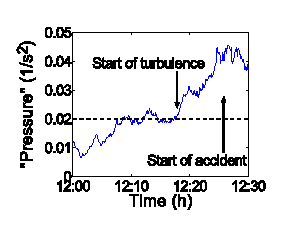
\includegraphics[width=0.5\linewidth]{Pressure.eps}
    \caption{The pressure leading up the the crowd disaster in Mina/Makkah during the Hajj in 1426H on January 12, 2006 \cite{empircalstudy}}
    \label{mekkahCrowdDistaster206}
\end{figure}

\sinote{Det kunne være fedt hvis vi skriver nøjagtigt hvad grænseværdier er for de 4 faktorer. Se fruin Crowd distasters - A systems evaluation of causes and countermeasures (1981)}

\subsection{Summary}\label{sec:crowd_conditions_summary}

\sinote{Write conclusion and use below pros, cons list}

\subsubsection{Density}

%\begin{minipage}[t]{0.46\linewidth}
%    \centering Pros
%    \begin{itemize}
%        \item Good for determining how easy it is to pass through an area
%    \end{itemize}
%\end{minipage}%
%\begin{minipage}[t]{0.46\linewidth}
%    \centering Cons
%    \begin{itemize}
%        \item Can be misleading regarding the danger level of a crowd since a high density of people is not dangerous on its own. Low density areas can be more dangerous than high density areas for the people in it
%    \end{itemize}
%\end{minipage}\par\bigskip

\paragraph{Pros}
\begin{itemize}
    \item Good for determining how easy it is to pass through an area
\end{itemize}

\paragraph{Cons}
\begin{itemize}
    \item Can be misleading regarding the danger level of a crowd since a high density of people is not dangerous on its own. Low density areas can be more dangerous than high density areas for the people in it
\end{itemize}

\subsubsection{Velocity}

%\begin{minipage}[t]{0.46\linewidth}
%    \centering Pros
%    \begin{itemize}
%        \item Can help predict how distribution of density will change
%    \end{itemize}
%\end{minipage}%
%\begin{minipage}[t]{0.46\linewidth}
%    \centering Cons
%    \begin{itemize}
%        \item Hard to represent
%        \item It can easily be mistaken for turbulence and vice versa
%        \item It implies a crowd movement tendency that does not necessarily hold. To increase precision of crowd movement predictions other characteristics such as paths, buildings and previous patterns should also considered
%    \end{itemize}
%\end{minipage}\par\bigskip

\paragraph{Pros}
\begin{itemize}
    \item Can help predict how distribution of density will change
\end{itemize}

\paragraph{Cons}
\begin{itemize}
    \item Hard to represent
    \item It can easily be mistaken for turbulence and vice versa
    \item It implies a crowd movement tendency that does not necessarily hold. To increase precision of crowd movement predictions other characteristics such as paths, buildings and previous patterns should also considered
\end{itemize}

\subsubsection{Turbulence}

%\begin{minipage}[t]{0.46\linewidth}
%    \centering Pros
%    \begin{itemize}
%        \item Useful as an early indicator of potential crowd control situations
%    \end{itemize}
%\end{minipage}%
%begin{minipage}[t]{0.46\linewidth}
%    \centering Cons
%    \begin{itemize}
%        \item Can be hard to infer from visual observation
%        \item Easy to misinterpret as movement velocity and flow direction
%    \end{itemize}
%\end{minipage}\par\bigskip

\paragraph{Pros}
\begin{itemize}
    \item Useful as an early indicator of potential crowd control situations
\end{itemize}

\paragraph{Cons}
\begin{itemize}
    \item Can be hard to infer from visual observation
    \item Easy to misinterpret as movement velocity and flow direction
\end{itemize}

\subsubsection{Pressure}

%\begin{minipage}[t]{0.46\linewidth}
%    \centering Pros
%    \begin{itemize}
%        \item Very useful for finding potential dangerous situations in a crowd
%        \item Tested and documented quantifiable limit for dangerous environments
%    \end{itemize}
%\end{minipage}%
%\begin{minipage}[t]{0.46\linewidth}
%    \centering Cons
%    \begin{itemize}
%        \item Hard to calculate
%        \item Easy to misinterpret as movement velocity and flow direction
%    \end{itemize}
%\end{minipage}\par\bigskip

\paragraph{Pros}
\begin{itemize}
    \item Very useful for finding potential dangerous situations in a crowd
    \item Tested and documented quantifiable limit for dangerous environments
\end{itemize}

\paragraph{Cons}
\begin{itemize}
    \item Hard to calculate
    \item Easy to misinterpret as movement velocity and flow direction
\end{itemize}